%
% Documento: Metodologia
%

\chapter{Metodologia}\label{chap:Metodologia} 
A metodologia foi composta de quatro fases, onde a primeira é constituída da aplicação de um questionário para analisar o interesse em relação a proposta e o perfil da comunidade acadêmica, buscando entender quais as necessidades existentes relacionadas a Mobilidade Urbana do Campus Macapá.% Está fase irá deixar claro qual é o problema existente e, qual à importância da solução.

A segunda fase realizou-se mediante revisão teórica sobre o que fundamenta soluções de mobilidade, qual é a sua área de estudo e o que trazem de benefícios no ambiente de Mobilidade Urbana.

Na terceira fase foi realizada uma pesquisa na qual o objetivo foi encontrar soluções de Mobilidade Inteligente de todo tipo. Após, buscamos pela solução que apresentasse condições para que pudéssemos realizar testes e que tivesse características de serviços de caronas, transporte e compartilhamento de viagens. \mnote{Aqui podes dizer também que nessa busca era importante encontrarmos algo que pudessemos testar no cenário da unifap, ou que tivessemos alguma liberdade para mudanças. Levando em condideração que transportes privados gerariam custos ao passaageiro e o objetivo aqui é justamente a colaboração por meio de caronas. }

A quarta fase foi iniciada a implementação da solução inteligente com uso dos serviços em nuvem. Ajustes necessários foram feitos, como contextualizar os endereços da cidade de Macapá e o Campus Macapá dentro da solução inteligente. \mnote{Optou-se por uma solução que podessemos realizar ajustes, realizar sua implementação e realizarmos ajustes necessários.} 

E para finalizar, foi dirigido um questionário para  validação do uso da solução por alguns participantes da pesquisa, que responderam perguntas em escalas likert e subjetivas, visando a validação do mesmo, assim como, possíveis contribuições. 

Será realizada a escrita do documento de TCC de forma concomitante as fases mencionadas acima.


\begin{comment}
	Para a realização do estudo sobre CI focado em Mobilidade Inteligente, realizou-se uma revisão de literatura considerando os trabalhos publicados nos últimos vinte anos. A partir destes trabalhos, selecionou-se as soluções de Mobilidade Inteligente encontradas, como também se fez uma busca de aplicativos que propõem soluções de mobilidade com o objetivo de analisar sua proposta e suas funcionalidades. 
	
	A etapa seguinte deste projeto realizou uma pequisa com a comunidade acadêmica da Unifap utilizando um questionário \textit{online}.
	%... 
	A coleta de dados foi realizada baseado em um questionário com 21 perguntas construído na ferramenta Google Forms da google e compartilhado em grupos de WhatsApp, Facebook, Instagram e em papéis de divulgação espalhados por vários blocos da UNIFAP - campus Macapá. %
	
	Assim, realizou-se um levantamento com uma abordagem quantitativa dos dados descrevendo os resultados das perguntas realizadas, considerando mobilidade e quais tecnologias auxiliaram e quando passaram a implementá-las nos serviços de mobilidade. 
	
	A partir das etapas anteriores, o projeto focou na análise comparativa de diferentes tipos soluções de mobilidade para a comunidade acadêmica da Unifap e, foi realizada a análise de requisitos das soluções mais viáveis analisadas nas etapas anteriores. 
	
	As etapas seguintes pretendem focar na análise de viabilidade e implementação e utilização das soluções existentes e as dificuldades de implementação e utilização, e se existir viabilidade, propor a sua implementação com objetivo de ajudar a comunidade acadêmica em geral, lhes dando uma alternativa de mobilidade inteligente baseada em todo um estudo local.
	
\end{comment}


\begin{comment} %orientações da professora inicio
\textbf{NOTA - TEM SEMPRE EM MENTE OS "PASSOS" QUE VAIS SEGUIR:}
\textit{
\begin{itemize}
    \item Entender o perfil da comunidade acadêmica e os problema enfrentados;
\item Estudar as solução de mobilidade existentes considerando o conceito de cidades inteligentes
\item Propor uma solução para a comunidade acadêmica da Unifap (que considere o perfil da comunidade acadêmica, os problemas enfrentados e a realidade do contexto local (Macapá e seus problemas estruturais, e a Unifap). 
\end{itemize}
}
\textbf{NOTA - NÃO ESQUECER:}
\textit{Não fazer nenhuma afirmação sem dados e provas.}

O processo inicial foi realizada por meio de uma entrevista ...
\end{comment}
%Será desenvolvido inicialmente um protótipo do aplicativo de caronas, com as principais funcionalidades e será entre a pesquisa de aceitação, onde foi 





\begin{comment} % comentário sobre o levantamento histórico
%
	\mnote{Patrícia: Aqui vais falar do segundo "passo" e tens um objetivo bem claro que ele também. Não tirar isso do foco.}
levantamento histórico da mobilidade e da tecnologia que auxilia a mobilidade desde o início e um breve comentário sobre, análise dos dados adquiridos na pesquisa, com o perfil dos possíveis usuários em relação a carona solidária, e o quantitativo de possíveis caronas e “caroneiros”.

\end{comment}    % fim

\begin{comment} %essa parte não tem que estar aqui. Coloca na parte de resultados preliminares
Dos pontos importantes a serem mencionados que foram obtidos no questionário é a respeito da segurança, a maior parte dos entrevistados do questionário disseram que “Sim” quando perguntado se faria diferença do aplicativo ser acessado apenas por pessoas que têm vínculo com a instituição.


\begin{figure}[!hbtp]
	\centering
	\caption{Percepção}
	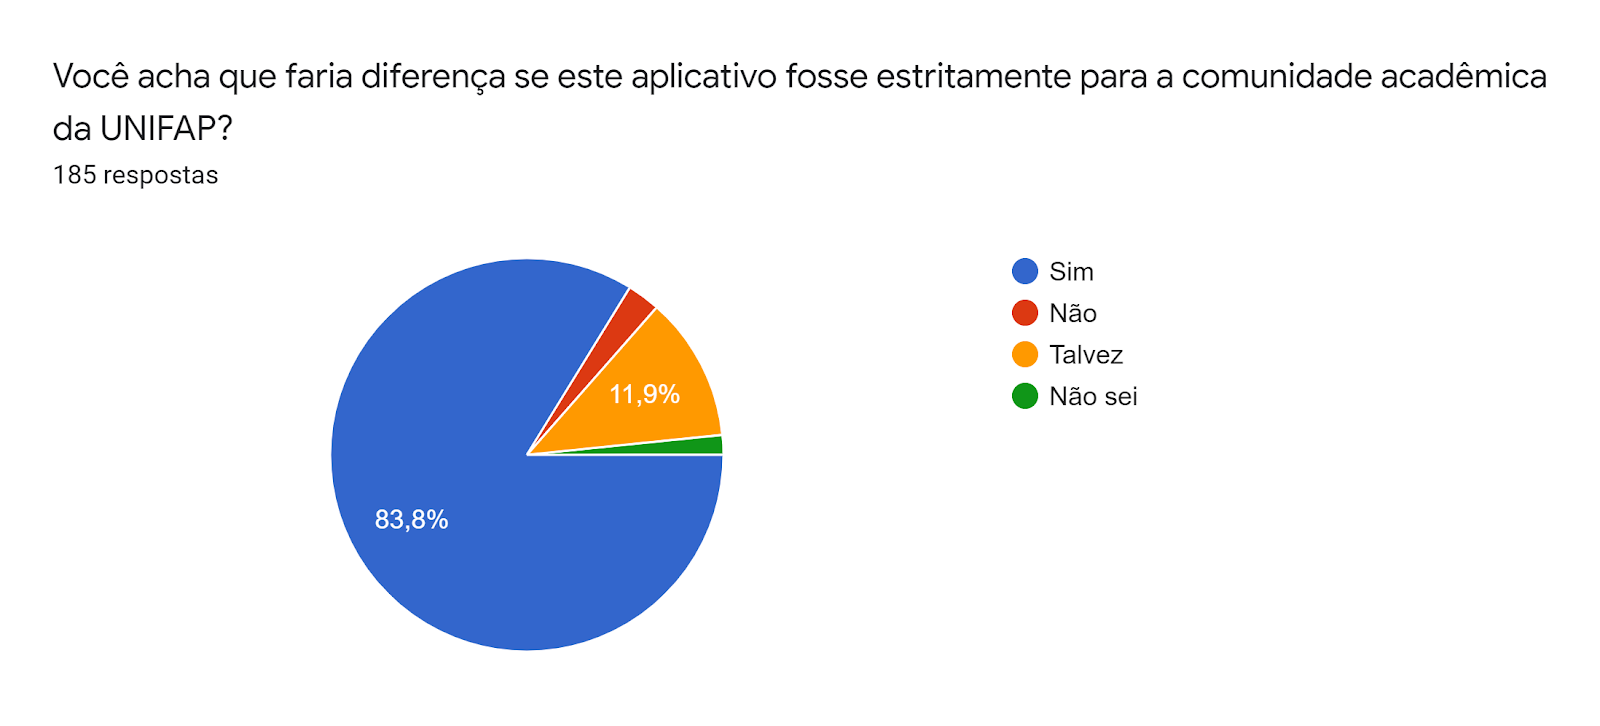
\includegraphics[width=12cm]{./04-figuras/questionario/18.png}
	\label{percepcao}
	\fonte{Elaborado pelo autor}
\end{figure}

\end{comment} %até aqui vai para a seção "resultados preliminares"


%Assim, será definido a metodologia em 3 passos:

% comentado para não aparecer no compilado
	%\mnote{Patrícia: a partir daqui vais falar do terceiro "passo". Ajusta o texto.}
    %
%No terceiro passo realizei o levantamento de requisitos para apresentar um protótipo funcional, desde requisitos funcionais, como o criação de caronas que será restrito apenas para pessoas vinculadas à instituição.

%\textbf{Aqui vai o texto para falar dos passos do caronaê, da apresentação das telas do caronaê}% 

%No terceiro passo detalharei as telas e funcionalidades do aplicativo Caronaê, apresentarei os serviços pensados e utilizados na proposta tanto do projeto Caronaê e quais deles foram reutilizados para a proposta na Unifap.



\begin{comment} % está parte era da proposta de criação do app ou do mockup

\textbf{Foi escrito quando a ideia era criar um app ou um mockup bem traabalhado}
O segundo passo será a construção do UX (User Experience) e UI (User Interface) no software Adobe XD para colocar em prática as primeiras ideias de design do aplicativo, a interface, cores, logo, funcionalidades, entre outros. E para concluir, o quarto passo é os testes, onde será avaliado se as funcionalidades iniciais, junto a isso, estarei finalizando a escrita do documento de trabalho de conclusão de curso.

\textbf{NOTA: MA COISA INTERESSANTE QUE A LORENA FEZ FOI SEPARAR A METODOLOGIA EM "ETAPAS CONCLUÍDAS" E "ETAPAS PENDENTES". VOU CRIAR AS SEÇÕES ABAIXO COMO ELA CRIOU E VC ORGANIZA DIREITINHO.}

\begin{itemize}
\item Questionário
\item Analise dos dados coletados no questionário 
%(parcialmente)
\item Levantamento histórico sobre mobilidade, mobilidade inteligente, campus e cidades inteligentes %(parcialmente, dissertar mais a frente do texto sobre)
\item Levantamento das soluções de mobilidade inteligente
\item Triagem das soluções inteligentes encontradas
\item Primeiros testes com os serviços fornecidos pelo projeto Caronae
\item Teste com o serviço backend do Caroonaê
\item Teste com o aplicativo Android do Caronaê
\item Adequação para testes no código Java do aplicativo Caronaê
\item Levantamento dos requisitos iniciais do aplicativo Caronaê
\item Inclusão das Zonas e bairros da cidade de Macapá no backend do serviço Caronaê
\item Mudança do texto dos campos que estavam UFRJ para UNIFAP
\end{itemize}

\section{Etapas pendentes}

\begin{itemize}
\item Adicionar todos os requisitos da solução esolhida
\item Escrita do trabalho de conclusão final
\end{itemize}

\end{comment}
